\iffalse
PICAT inoltre prevede anche alcuni aspetti funzionali. A parte permettere la definizione di funzioni ricorsive, queste possono essere definite tramite l'utilizzo di pattern matching. Oltre a ciò PICAT prevede una serie di funzioni già pronte per la manipolazione delle liste ed una certa facilità a modificarle. PICAT prevede inoltre un limitato supporto alle funzioni higher order: non se ne possono creare di nuove infatti, come in un qualsiasi linguaggi funzionale, ma ne prevede un insieme già creato. L'uso di queste funzioni è scoraggiato nel caso in cui si voglia creare programmi efficienti poichè creano un overhead elevato
\fi

\begin{frame}{Programmazione funzionale}

	\begin{figure}
		\hfill
		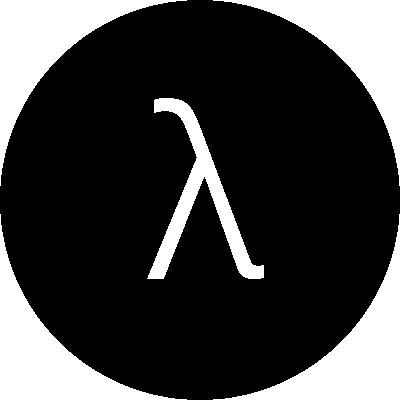
\includegraphics[scale=0.1]{res/lambda}
	\end{figure}

	\begin{itemize}
		\item Funzioni ricorsive
		\item Pattern matching per la definizione di funzioni
		\item Facilità a manipolare le liste (funzioni built-in e comprehension)
		\item Limitato supporto alle funzioni higher-order
			\begin{itemize}
				\item \texttt{apply}, \texttt{call}, \texttt{foldl}, \texttt{map}...
				\item Uso scoraggiato a causa dell'overhead elevato
			\end{itemize}
	\end{itemize}

	\begin{figure}
		\hspace*{-7cm}
		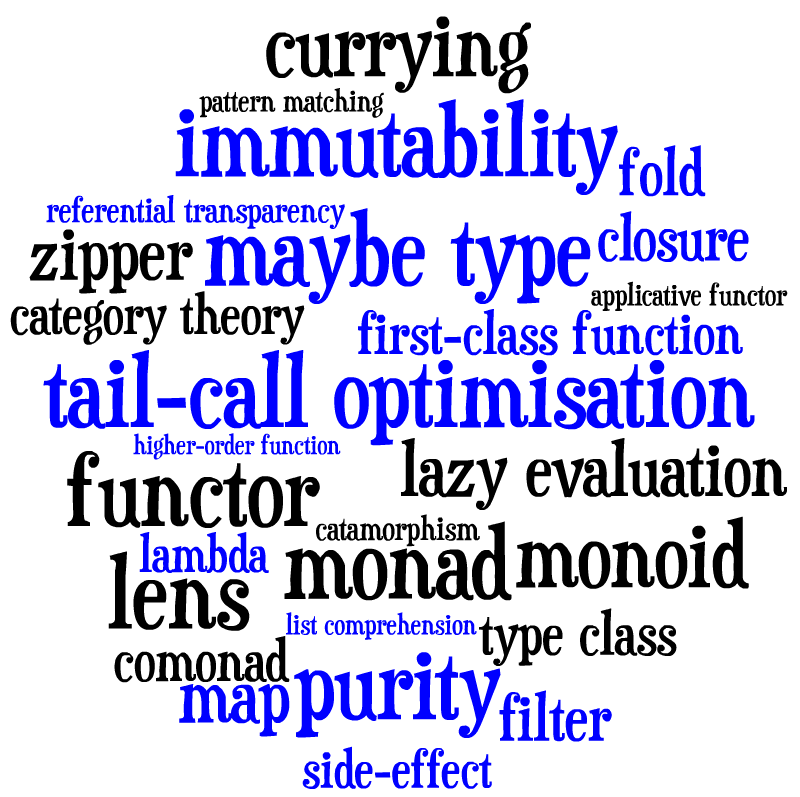
\includegraphics[scale=0.1]{res/functional}
	\end{figure}

\end{frame}